\section{Desenho da Arquitetura e Dinâmica Matemática}
\label{sec:arquitetura}

\subsection{Representação Explícita em Grafo Direcionado (\texttt{nx.DiGraph})}
Diferentemente de implementações matriciais opacas, a classe \texttt{MLPGraph} (\texttt{code/mlp/core\_mlp/graph.py}) instancia cada neurônio e cada sinapse como entidades explícitas de um grafo direcionado $G = (V, E)$, conforme ilustrado no desenho arquitetural da Figura~\ref{fig:arquitetura_diagrama}.

\begin{figure}[H]
    \centering
    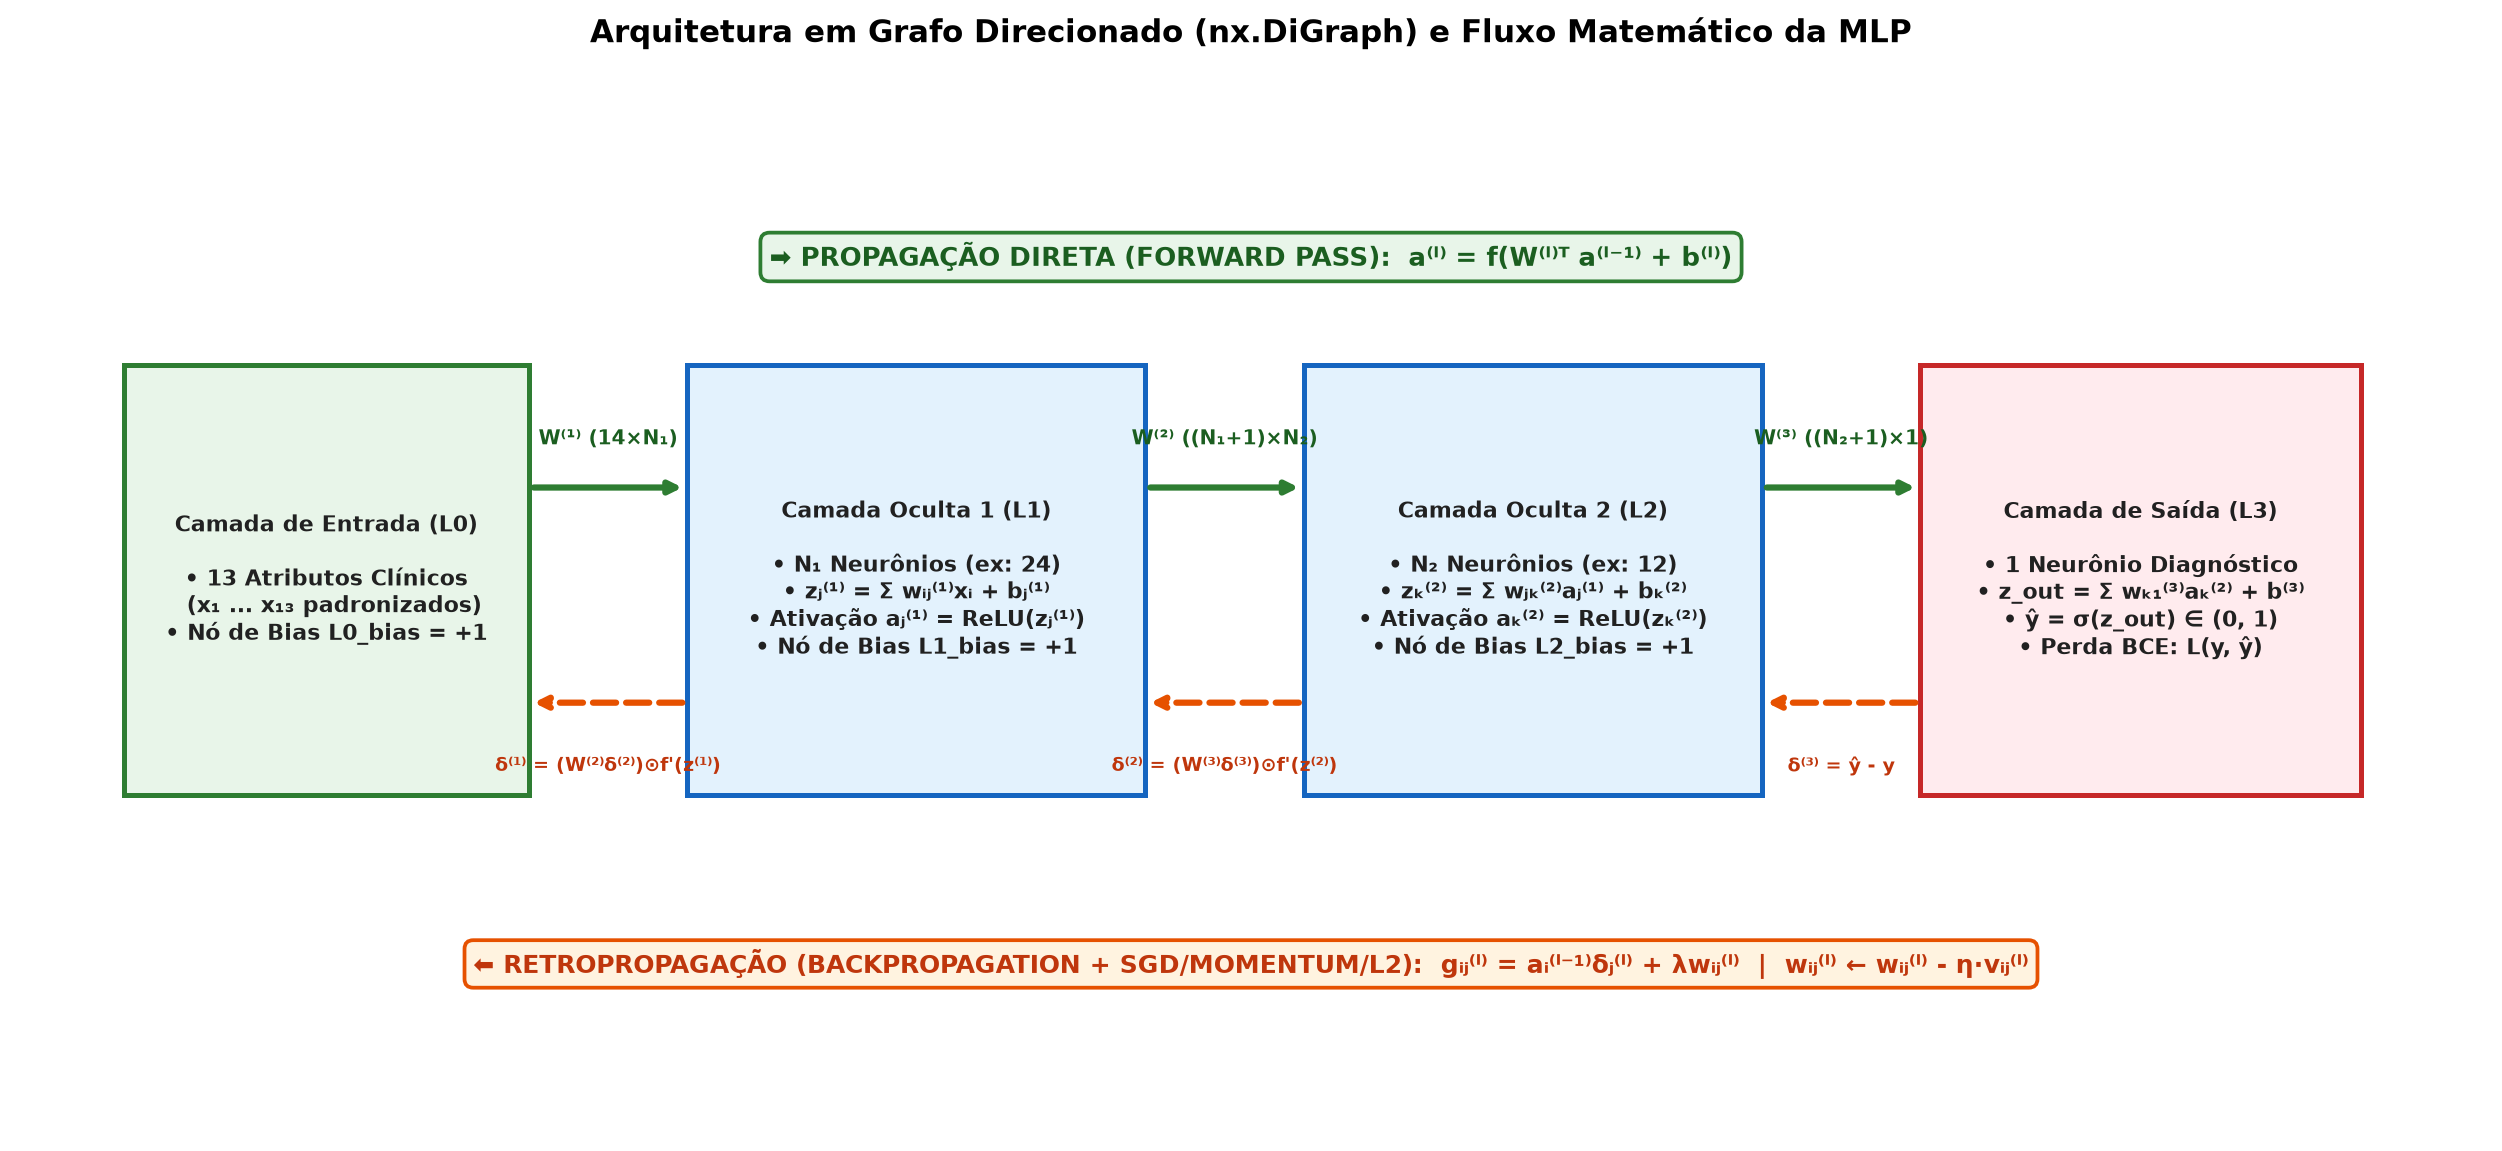
\includegraphics[width=0.98\textwidth]{figs/arquitetura_diagrama.png}
    \caption{Desenho da arquitetura da MLP em grafo direcionado (\texttt{nx.DiGraph}) e fluxo matemático bidirecional (\textit{Forward Pass} e \textit{Backpropagation}).}
    \label{fig:arquitetura_diagrama}
\end{figure}

O funcionamento estrutural do grafo organiza-se em três componentes:
\begin{itemize}
    \item \textbf{Vértices Neurais (\texttt{L\{l\}\_N\{j\}}):} cada neurônio $j$ da camada $l \in \{0, \dots, L-1\}$ armazena os atributos \texttt{z} (potencial pré-ativação $z_j^{(l)}$), \texttt{value} (ativação $a_j^{(l)}$) e \texttt{delta} (erro retropropagado $\delta_j^{(l)}$).
    \item \textbf{Vértices de Bias (\texttt{L\{l\}\_bias}):} cada camada $l \in \{0, \dots, L-2\}$ possui um nó de bias explícito com ativação constante $a_{\text{bias}}^{(l)} = +1$, conectado a todos os neurônios da camada $l+1$. Essa modelagem corrige uma limitação da versão preliminar, na qual a primeira camada oculta carecia de termo de bias.
    \item \textbf{Arestas Sinápticas (\texttt{(u, v)}):} cada aresta direcionada armazena o peso sináptico atual \texttt{weight} ($w_{uv}$), o peso no início da época \texttt{prev\_weight} ($w_{uv}^{(t-1)}$), a variação líquida na época \texttt{delta\_weight} ($\Delta w_{uv}$), o gradiente instantâneo \texttt{gradient} ($\partial \mathcal{L}/\partial w_{uv}$) e a velocidade de momento \texttt{velocity} ($v_{uv}$).
\end{itemize}

\subsection{Propagação Direta (\textit{Forward Pass})}
Para cada amostra $\mathbf{x} \in \mathbb{R}^{13}$, os nós de entrada recebem $a_i^{(0)} = x_i$. Em seguida, para cada camada $l = 1, \dots, L-1$, calcula-se o potencial pós-sináptico e a ativação não linear:
\begin{equation}
    z_j^{(l)} = \sum_{i=1}^{N_{l-1}} w_{ij}^{(l)} a_i^{(l-1)} + b_j^{(l)}, \qquad a_j^{(l)} = f^{(l)}\!\left(z_j^{(l)}\right)
\end{equation}
Nas camadas ocultas, o sistema suporta sete funções de ativação configuráveis em tempo real (\texttt{ReLU}, \texttt{Leaky ReLU}, \texttt{Tanh}, \texttt{Sigmoide}, \texttt{ELU}, \texttt{SELU} e \texttt{ReLU6}). Na camada de saída ($L-1$), emprega-se a função sigmoide $\hat{y} = \sigma(z_{\text{out}}) = (1 + e^{-z_{\text{out}}})^{-1}$.

\subsection{Retropropagação (\textit{Backpropagation}) e Correção Analítica do Gradiente BCE}
A função objetivo adotada é a Entropia Cruzada Binária (\textit{Binary Cross-Entropy} -- BCE) com regularização $L_2$:
\begin{equation}
    \mathcal{L}(\hat{y}, y) = -\Big[y \ln(\hat{y}) + (1 - y)\ln(1 - \hat{y})\Big] + \frac{\lambda}{2}\sum_{l,i,j}\left(w_{ij}^{(l)}\right)^2
\end{equation}

Na revisão da versão preliminar, constatou-se que o sinal de erro na saída estava implementado como $(\hat{y} - y)\sigma'(z_{\text{out}})$, expressão correspondente à perda quadrática (MSE) que introduz saturação prematura quando $\hat{y} \to 0$ ou $\hat{y} \to 1$. Pela regra da cadeia aplicada à BCE, o termo $\hat{y}(1-\hat{y})$ cancela-se exatamente:
\begin{equation}
    \delta^{(L-1)} = \frac{\partial \mathcal{L}}{\partial z_{\text{out}}} = \left(\frac{\hat{y} - y}{\hat{y}(1 - \hat{y})}\right)\hat{y}(1 - \hat{y}) = \hat{y} - y
\end{equation}

Para as camadas ocultas $l = L-2, \dots, 1$, o erro é retropropagado pelas arestas sucessoras de cada nó:
\begin{equation}
    \delta_j^{(l)} = \left(\sum_{k=1}^{N_{l+1}} w_{jk}^{(l+1)} \delta_k^{(l+1)}\right) f'^{(l)}\!\left(z_j^{(l)}\right)
\end{equation}
Por fim, os pesos são atualizados por Gradiente Descendente com \textit{Momentum} ($\beta$) e decaimento $L_2$ ($\lambda$):
\begin{equation}
    g_{ij}^{(l)} = a_i^{(l-1)}\delta_j^{(l)} + \lambda w_{ij}^{(l)}, \qquad v_{ij}^{(l)} \leftarrow \beta v_{ij}^{(l)} + g_{ij}^{(l)}, \qquad w_{ij}^{(l)} \leftarrow w_{ij}^{(l)} - \eta_t v_{ij}^{(l)}
\end{equation}
